\documentclass[11pt,a4paper]{article}

\usepackage[utf8]{inputenc}
\usepackage[T1]{fontenc}
\usepackage[english]{babel}
\usepackage{geometry}
\usepackage{microtype}
\usepackage{booktabs}
\usepackage{array}
\usepackage{longtable}
\usepackage{enumitem}
\usepackage{graphicx}
\usepackage{xcolor}
\usepackage{tikz}
\usepackage{pgfplots}
\usepackage{hyperref}
\usepackage[numbers,sort&compress]{natbib}
\usepackage{listings}
\usepackage{multirow}
\usepackage{amsmath}
\usetikzlibrary{arrows.meta,positioning,fit,shapes.geometric,calc}
\pgfplotsset{compat=1.18}

\geometry{margin=2.6cm}
\setlist{noitemsep,topsep=4pt}

\newcommand{\aidb}{AI-DB-Creator}
\definecolor{aidbblue}{HTML}{1F4E79}
\definecolor{aidbcyan}{HTML}{D9EAF7}
\definecolor{aidbgreen}{HTML}{DDEBDD}
\definecolor{aidborange}{HTML}{FCE4D6}
\definecolor{aidbgray}{HTML}{F2F2F2}
\tikzset{
  box/.style={rounded corners, draw=aidbblue, thick, fill=aidbcyan, align=center, minimum height=0.9cm, text width=3.0cm, font=\small},
  data/.style={rounded corners, draw=black!55, thick, fill=aidbgray, align=center, minimum height=0.9cm, text width=2.8cm, font=\small},
  agent/.style={rounded corners, draw=aidbblue, thick, fill=aidbgreen, align=center, minimum height=0.9cm, text width=2.8cm, font=\small},
  evalbox/.style={rounded corners, draw=black!60, thick, fill=aidborange, align=center, minimum height=0.9cm, text width=2.8cm, font=\small},
  arrow/.style={-{Latex[length=2.2mm]}, thick, draw=black!70}
}
\newcommand{\authoraction}[1]{%
  \vspace{0.6em}
  \noindent\framebox[\linewidth][l]{%
    \begin{minipage}{0.95\linewidth}
    \textbf{Author action required.} #1
    \end{minipage}}
  \vspace{0.6em}
}
\newcommand{\surveyplaceholder}[2]{%
  \vspace{0.4em}
  \noindent\colorbox{aidborange}{%
    \begin{minipage}{0.95\linewidth}
    \textbf{[SURVEY / EXPERIMENT REQUIRED] #1}\newline
    \textit{#2}
    \end{minipage}}
  \vspace{0.4em}
}

\lstdefinelanguage{json}{
  basicstyle=\ttfamily\small,
  morestring=[b]",
  stringstyle=\color{aidbblue},
  showstringspaces=false,
}

\title{\textbf{\aidb: an LLM-powered visual interface for automatic database schema generation and population from heterogeneous documents}}

\author{
  Author name to be confirmed\\
  \small Affiliation to be confirmed\\
  \small \texttt{email to be confirmed}
  \and
  Co-authors to be confirmed
}

\date{\today}

\begin{document}
\maketitle

\begin{abstract}
The design of a relational database schema and the population of its tables remain technical tasks that require expertise in data modelling, normalisation, and SQL. This prevents non-expert users---domain experts, researchers, small-business operators---from autonomously structuring and querying their data. This paper presents \aidb, a research platform that combines Large Language Models (LLMs) with an interactive visual interface to enable users with no database background to generate, populate, and explore relational databases. The system accepts heterogeneous documents (CSV, Excel, PDF, TXT, SQL) and natural-language descriptions, and guides the user through five phases: document ingestion, LLM-based schema generation (normalised tables, primary/foreign keys, constraints), automatic database creation and migration, deterministic-first hybrid population from source documents, and a visual data environment with search, filtering, inline editing, CRUD operations, and multi-dialect export (SQLite, PostgreSQL, MySQL, MSSQL). Backup-and-restore snapshots and operation-history metadata provide safety and traceability.

The paper describes the architecture, schema prompting and deterministic-first hybrid population, the multi-dialect import/export pipeline, and a comprehensive evaluation protocol structured around four research questions. These investigate schema quality (normalisation, key identification F1), population accuracy (cell-level precision/recall), the impact of human-in-the-loop validation (three-arm experiment with Raw NASA-TLX and SUS), and user interaction patterns (log sequence mining and clustering). Sections that require empirical data are explicitly marked with collection instructions.
\end{abstract}

\noindent\textbf{Keywords:} Large Language Models; database schema generation; automatic data population; visual interface; human-in-the-loop; non-expert users; multi-dialect export; CRUD; normalisation.

\section{Introduction}
Relational databases remain the dominant paradigm for structured data storage in business, research, and government. Their creation, however, requires a combination of skills---data modelling, normalisation theory, SQL proficiency---that is rarely found outside specialised technical roles. According to surveys of small and medium enterprises, a significant fraction of data management is still performed through spreadsheets precisely because the leap from flat tabular data to a normalised relational schema is perceived as too costly or technically demanding~\citep{bernstein2011spreadsheets}. This gap creates friction: data that could be queried, related, and analysed remains locked in isolated documents, and the benefits of structured storage---integrity constraints, efficient joins, standardised access---are lost.

Recent advances in Large Language Models (LLMs) have opened new possibilities for lowering the technical barriers to database creation. LLMs have demonstrated remarkable capabilities in code generation~\citep{chen2021evaluating}, text-to-SQL translation~\citep{yu2018spider}, schema matching~\citep{zhang2023schema}, and structured data extraction~\citep{narayan2022data}. However, existing research has focused on individual sub-tasks in isolation. No prior work, to the best of our knowledge, addresses the complete end-to-end problem: going from a set of heterogeneous, unstructured or semi-structured documents to a fully populated, normalised relational database through a unified workflow accessible to non-experts.

This paper presents \aidb, a research platform designed to fill this gap. \aidb\ combines an LLM-based generation engine with a visual interactive interface to support users without database expertise through the entire lifecycle of database creation. The key contributions of this work are:

\begin{enumerate}
  \item \textbf{An end-to-end pipeline} that transforms heterogeneous documents (CSV, XLSX, PDF, TXT, SQL) into a normalised relational database through a guided five-phase workflow: ingestion, schema generation, database creation, data population, and exploration.
  \item \textbf{A deterministic-first hybrid population strategy} that separates schema inference from extraction. CSV/Excel headers are matched by normalised rules before semantic LLM mapping is considered; unstructured sources use an LLM fallback against the generated schema.
  \item \textbf{A multi-dialect export engine} supporting four SQL dialects---SQLite, PostgreSQL, MySQL, MSSQL---with automatic type mapping and referentially safe DDL generation.
  \item \textbf{An evaluation framework} comprising four research questions, each with quantitative metrics and a detailed data-collection protocol. The framework covers schema quality (RQ1), population accuracy (RQ2), human-in-the-loop validation impact (RQ3), and user interaction patterns (RQ4).
  \item \textbf{A reproducible research infrastructure} with full source code, documentation suite, and versioned artifacts available in the project repository.
\end{enumerate}

The paper is structured as follows. Section~\ref{sec:background} reviews related work in LLMs for databases, schema generation, and human-in-the-loop tools. Section~\ref{sec:system} describes the system architecture, frontend and backend components, and the LLM integration strategy. Section~\ref{sec:workflow} presents the workflow in detail, with examples of the prompting pipelines. Section~\ref{sec:rq} defines the research questions and hypotheses. Section~\ref{sec:eval} describes the evaluation protocol, including datasets, participants, metrics, and statistical methods. Section~\ref{sec:results-placeholder} outlines the expected results and analysis plan. Section~\ref{sec:threats} discusses threats to validity. Section~\ref{sec:discussion} frames the expected contributions and limitations. Section~\ref{sec:conclusion} concludes. Throughout the paper, sections that depend on experimental data are marked with \textbf{[SURVEY / EXPERIMENT REQUIRED]} and include precise instructions for data collection.

\section{Background and related work}
\label{sec:background}
\subsection{LLMs for database-related tasks}
The application of LLMs to database tasks has grown rapidly. The most mature area is text-to-SQL translation, where models translate natural-language questions into SQL queries. Benchmarks such as Spider~\citep{yu2018spider}, WikiSQL, and BIRD have driven progress, with models now exceeding 85\% execution accuracy on held-out examples. However, text-to-SQL assumes that the database schema already exists; it does not address schema design.

Schema matching---identifying correspondences between columns of different tables---has also benefited from LLM capabilities~\citep{zhang2023schema}. LLM-based matchers outperform traditional similarity-based approaches on benchmark datasets, but they operate on existing schemas rather than generating new ones.

Data cleaning and transformation have been explored through LLM-based approaches for entity resolution, missing-value imputation, and format standardisation~\citep{narayan2022data}. These techniques are relevant to the population phase of \aidb, where extracted values may need type coercion or deduplication.

\subsection{Schema generation from natural language}
The task of generating a database schema from a natural-language description has received less attention. Early work by~\citet{chaudhuri2023nl2schema} proposed NL2Schema, a system that translates natural-language descriptions into CREATE TABLE statements using few-shot prompting. However, that system operates on single-table descriptions and does not handle multi-table normalisation, foreign-key inference, or integration with source documents.

Reverse-engineering approaches infer schemas from data sources~\citep{rahm2010schema}. These methods analyse the structure of CSV files or spreadsheets to propose column types and potential keys, but they cannot infer relationships across files or enforce normalisation beyond what is evident from the data layout.

\aidb\ differs from both approaches by combining natural-language prompting with document content. The LLM receives both a high-level description of the domain and the actual text extracted from the user's documents, enabling it to propose a schema that is both structurally sound and semantically aligned with the data.

\subsection{Human-in-the-loop database tools}
Visual database design tools have existed for decades: MySQL Workbench, ER/Studio, dbdiagram.io, and others provide graphical environments for entity-relationship modelling. These tools are powerful for users who understand normalisation, cardinality, and key selection, but they assume the very expertise that \aidb\ aims to replace. For non-expert users, the challenge is not the graphical notation but the underlying model of what constitutes a well-designed schema.

The human-in-the-loop paradigm has been studied in the context of interactive machine learning~\citep{fails2003interactive,amershi2014power}, where user feedback is used to refine model outputs. In the database domain,~\citet{hellerstein2020interactive} explored interactive data cleaning, showing that user involvement improves data quality. \aidb\ applies this paradigm to schema generation: the LLM proposes a schema, and the user can review, edit, add, or remove elements through an intuitive interface before the database is created.

\subsection{Retrieval-Augmented Generation for structured data}
RAG~\citep{lewis2020rag} combines a generative model with indexed external memory. While most RAG applications focus on question answering over unstructured text, the paradigm is also applicable to structured data. In \aidb, the RAG concept appears in two forms. First, the schema generation prompt includes the full document text as retrieved context. Second, the population prompt uses the generated table definitions as a structured target schema and the document text as the source from which values must be extracted. This dual application of the RAG principle---unstructured context for design, structured target for extraction---is, to our knowledge, novel.

\surveyplaceholder{RQ1 / RQ2 Literature gap confirmation}{Conduct a systematic literature review using the following search strings: ("LLM" OR "large language model") AND ("schema generation" OR "database creation" OR "automatic schema design"); ("LLM" OR "large language model") AND ("data population" OR "table population" OR "data extraction" AND "relational"). Document: (1) number of relevant papers found, (2) which sub-steps each paper covers, (3) datasets used for evaluation, (4) whether any existing work covers the full end-to-end pipeline. If any system covers both schema generation and population from heterogeneous documents, describe it in detail and explain how \aidb\ differs.}

\section{System architecture}
\label{sec:system}
\aidb\ follows a client-server architecture with a clear separation of concerns between the visual interface and the core logic.

\subsection{Overall architecture}

\begin{figure}[htbp]
\centering
\resizebox{\linewidth}{!}{%
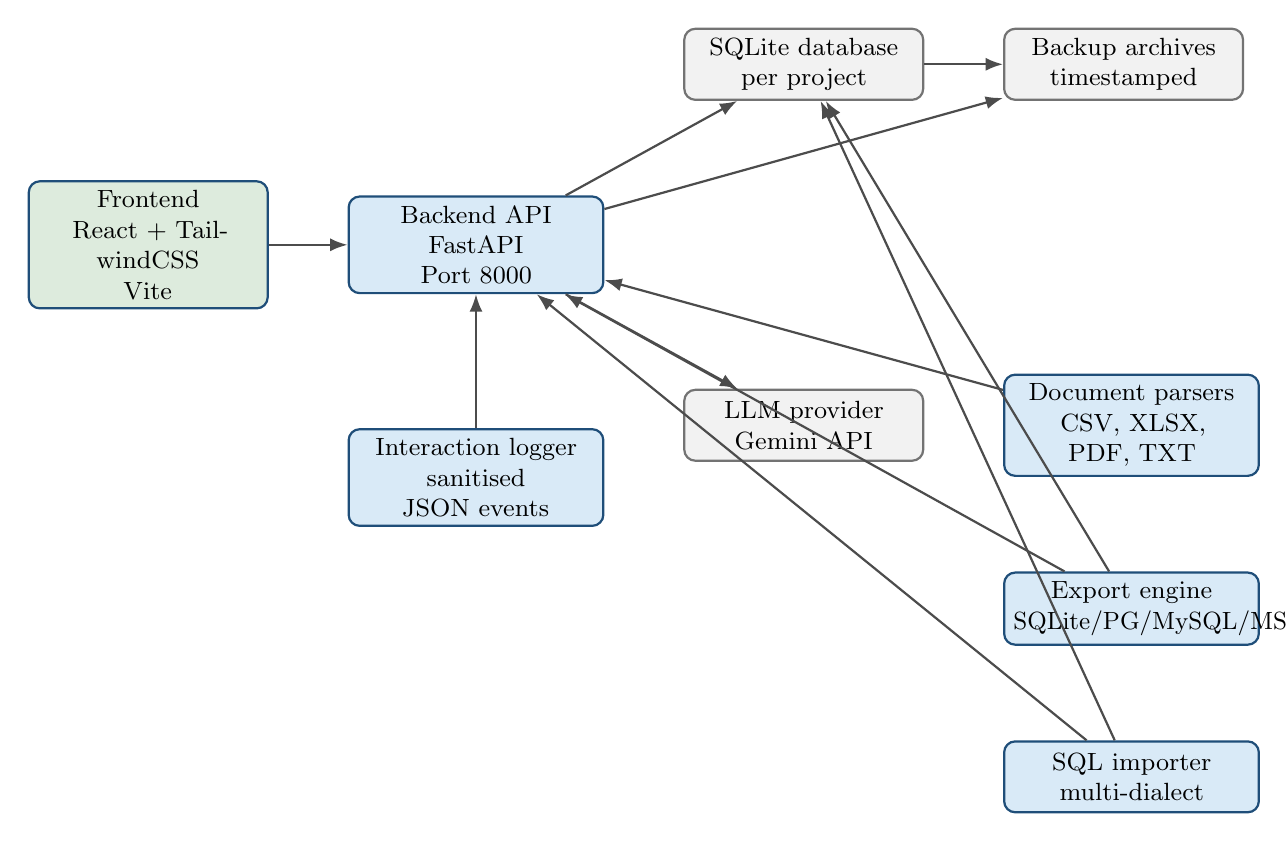
\begin{tikzpicture}[node distance=1.2cm and 1.0cm]
  \node[agent] (frontend) {Frontend\\React + TailwindCSS\\Vite};
  \node[box, right=of frontend] (api) {Backend API\\FastAPI\\Port 8000};
  \node[data, above right=of api] (db) {SQLite database\\per project};
  \node[data, right=of db] (backups) {Backup archives\\timestamped};
  \node[data, below right=of api] (llm) {LLM provider\\Gemini API};
  \node[box, right=of llm] (parser) {Document parsers\\CSV, XLSX, PDF, TXT};
  \node[box, below=of parser] (exporter) {Export engine\\SQLite/PG/MySQL/MSSQL};
  \node[box, below=of exporter] (importer) {SQL importer\\multi-dialect};
  \node[box, below=of api, yshift=-0.5cm] (logger) {Interaction logger\\sanitised JSON events};

  \draw[arrow] (frontend) -- (api);
  \draw[arrow] (api) -- (db);
  \draw[arrow] (api) -- (backups);
  \draw[arrow] (api) -- (llm);
  \draw[arrow] (parser) -- (api);
  \draw[arrow] (exporter) -- (api);
  \draw[arrow] (importer) -- (api);
  \draw[arrow] (logger) -- (api);
  \draw[arrow] (db) -- (backups);
  \draw[arrow] (exporter) -- (db);
  \draw[arrow] (importer) -- (db);
\end{tikzpicture}}
\caption{Overall architecture of \aidb. The backend is the central orchestrator, coordinating document parsing, LLM interaction, database operations, export/import, backup, and logging.}
\label{fig:architecture}
\end{figure}

The frontend is built with React 18, TypeScript, and Tailwind CSS, using Vite as the build tool. It communicates with the backend through a typed API client that wraps fetch calls. The frontend implements six main views: Dashboard (project listing and deletion), Schema (schema viewer, chat assistant, diagram, export/import controls), Data (table viewer with inline editing, search, filters, CSV export), Query (natural-language and direct SQL modes), Backup (snapshot management), and History (operation log).

The backend is built with FastAPI (tested on Python 3.10--3.13) and uses SQLAlchemy for database interactions. It exposes RESTful endpoints under the \texttt{/api} prefix. The backend is organised into eight service modules:
\begin{itemize}
  \item \textbf{schema\_service} — project CRUD, schema storage and retrieval, schema update with migration.
  \item \textbf{schema\_generation\_service} — LLM prompting for schema generation, response parsing.
  \item \textbf{population\_service} — LLM prompting for data extraction, row insertion, table creation.
  \item \textbf{backup\_service} — database file snapshot creation, listing, and restoration.
  \item \textbf{sql\_importer} — multi-dialect SQL CREATE TABLE parsing.
  \item \textbf{db\_export} — schema-only and full-database export to four SQL dialects.
  \item \textbf{interaction\_logger} — sanitised event logging for research-relevant operations and run manifests.
  \item \textbf{survey\_service} — survey configuration and response storage.
\end{itemize}

\subsection{Frontend component tree}

\begin{figure}[htbp]
\centering
\resizebox{0.85\linewidth}{!}{%
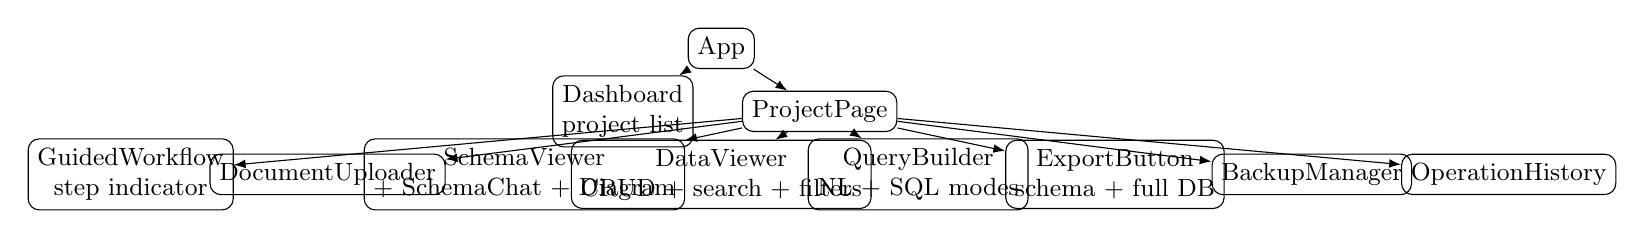
\begin{tikzpicture}[
  every node/.style={rounded corners, draw, font=\small, align=center},
  level distance=0.8cm,
  sibling distance=2.5cm,
  edge from parent/.style={draw, -{Latex[length=1.5mm]}}
]
\node {App}
  child {node {Dashboard\\project list}}
  child {node {ProjectPage}
    child {node {GuidedWorkflow\\step indicator}}
    child {node {DocumentUploader}}
    child {node {SchemaViewer\\+ SchemaChat + Diagram}}
    child {node {DataViewer\\CRUD + search + filters}}
    child {node {QueryBuilder\\NL + SQL modes}}
    child {node {ExportButton\\schema + full DB}}
    child {node {BackupManager}}
    child {node {OperationHistory}}
  };
\end{tikzpicture}}
\caption{Frontend component hierarchy. The ProjectPage component is the main workspace, containing eight child components.}
\label{fig:component-tree}
\end{figure}

\subsection{Document parsing layer}
The document parser supports five file formats:
\begin{itemize}
  \item \textbf{CSV} — uses Python's csv module; auto-detects delimiter and header row.
  \item \textbf{Excel (.xlsx)} — uses openpyxl; reads all sheets and concatenates text.
  \item \textbf{PDF} — uses PyMuPDF (fitz); extracts text page by page.
  \item \textbf{TXT} — direct UTF-8 text extraction.
  \item \textbf{SQL} — reads CREATE TABLE statements for schema import (not parsed for population).
\end{itemize}
Each parser implements a common interface and returns both the raw text and metadata (filename, type, row count for tabular formats). The extracted text is passed to the LLM as context for schema generation and population.

\section{User workflow}
\label{sec:workflow}
\aidb\ guides the user through a structured five-phase workflow. Figure~\ref{fig:workflow} illustrates the phases and their dependencies.

\begin{figure}[htbp]
\centering
\resizebox{0.95\linewidth}{!}{%
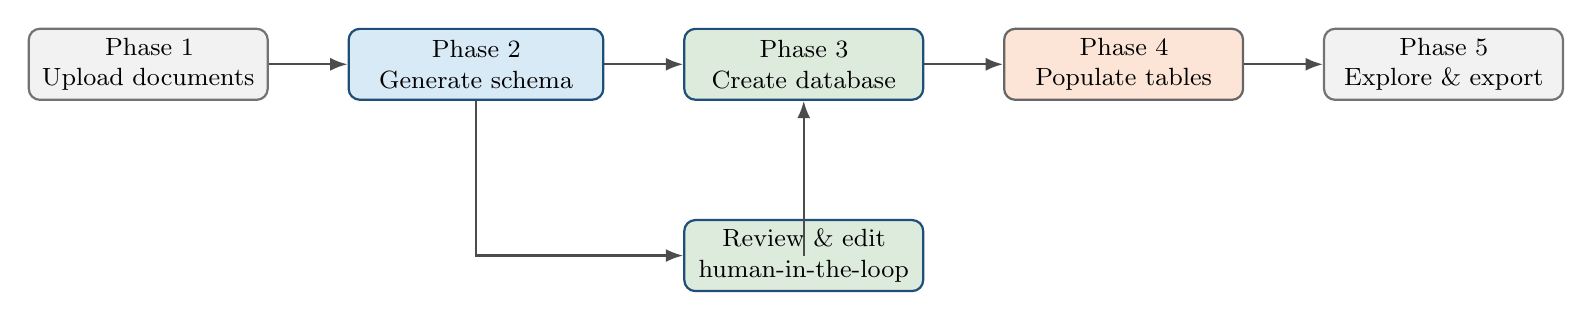
\begin{tikzpicture}[node distance=1.0cm and 1.0cm]
  \node[data] (upload) {Phase 1\\Upload documents};
  \node[box, right=of upload] (schema) {Phase 2\\Generate schema};
  \node[agent, right=of schema] (create) {Phase 3\\Create database};
  \node[evalbox, right=of create] (populate) {Phase 4\\Populate tables};
  \node[data, right=of populate] (explore) {Phase 5\\Explore \& export};
  \node[agent, below=1.5cm of create] (review) {Review \& edit\\human-in-the-loop};

  \draw[arrow] (upload) -- (schema);
  \draw[arrow] (schema) -- (create);
  \draw[arrow] (create) -- (populate);
  \draw[arrow] (populate) -- (explore);
  \draw[arrow] (schema) |- (review);
  \draw[arrow] (review) -| (create);
\end{tikzpicture}}
\caption{The five-phase user workflow. The review-and-edit loop (Phase 2b) is optional but recommended; it allows users to refine the schema before database creation.}
\label{fig:workflow}
\end{figure}

\subsection{Phase 1: Document ingestion}
The user creates a project and uploads documents. Supported formats are CSV, Excel, PDF, TXT, and SQL (for schema import). Each document is parsed and stored with metadata. The system displays a summary of uploaded documents with file type indicators.

\subsection{Phase 2: Schema generation}
The user triggers schema generation either through the chat interface (describing the desired database in natural language) or through the ``Quick Generate'' feature, which sends bounded document summaries (up to 5,000 characters per document in the current implementation) to the LLM with a structured prompt. The prompt instructs the LLM to:

\begin{enumerate}
  \item Identify the entities present in the documents and their attributes.
  \item Design a normalised relational schema aiming for 3NF.
  \item Define appropriate data types (INTEGER, TEXT, REAL, BOOLEAN, DATE, etc.).
  \item Identify primary keys (surrogate or natural).
  \item Identify foreign-key relationships between tables.
  \item Mark NOT NULL constraints where data implies mandatory values.
  \item Return the result as a JSON object.
\end{enumerate}

The LLM response is parsed into the internal \texttt{NormalizedSchema} model. A parsing failure is returned as a user-visible error; the current implementation does not perform an automatic corrected-prompt retry. The generated schema is displayed as a collection of table cards or as an entity-relationship diagram.

\subsection{Phase 2b: Human review and editing (optional)}
The user can review the generated schema and make changes:
\begin{itemize}
  \item Rename tables and columns.
  \item Add or remove columns.
  \item Change data types.
  \item Toggle primary-key and NOT NULL constraints.
  \item Add or remove foreign keys.
  \item Add or delete entire tables.
\end{itemize}
Changes are applied both to the in-memory schema and, after saving, to the physical SQLite database through migration (additive changes use ALTER TABLE; new tables are created).

\subsection{Phase 3: Database creation}
The schema is materialised as a SQLite database. If the database already exists (e.g.\ after a previous generation), the system compares old and new schemas and applies migration: new tables are created, new columns are added with ALTER TABLE, and data in existing columns is preserved.

\subsection{Phase 4: Data population}
Population follows a deterministic-first hybrid pipeline. For CSV and Excel sources, headers are normalised and matched against schema columns first; only unresolved headers are sent to the LLM for semantic mapping. Values remain tied to their source document and tabular coordinates. For unstructured PDF/TXT content, or when structured mapping yields no usable rows, the LLM extracts candidate rows against the target table definition. The fallback prompt includes:
\begin{itemize}
  \item The bounded text summary retained for each uploaded document.
  \item The table definition (column names, data types, NOT NULL constraints).
  \item An instruction to generate INSERT OR IGNORE statements.
  \item A rule forbidding NULL values for NOT NULL columns.
\end{itemize}
The response is validated and executed against the database. Each population run records its extraction method, source-document hashes, mapping confidence when algorithmically available, provider/model configuration and per-table inserted/skipped counts. A backup is automatically created before population to enable rollback.

\subsection{Phase 5: Data exploration and export}
The user can explore the populated data through the Data tab:
\begin{itemize}
  \item View each table with row counts.
  \item Search across all tables (global text search).
  \item Filter rows by column values.
  \item Edit cell values inline (with yellow highlighting for unsaved changes).
  \item Add new rows.
  \item Delete rows.
  \item Export table data as CSV.
\end{itemize}
The Export button supports:
\begin{itemize}
  \item Schema-only export (DDL) for all four dialects.
  \item Full-database export (DDL + INSERT statements) for all four dialects.
\end{itemize}

\subsection{Supporting features}
\begin{itemize}
  \item \textbf{Guided workflow stepper} — a four-step indicator showing the current phase and completeness status.
  \item \textbf{Backup manager} — manual labelled backups, automatic pre-destructive-operation backups, restore to any snapshot.
  \item \textbf{Operation history} — timestamped log of schema generations, populations, imports, backups, restores, queries, and data mutations. Export endpoints return artefacts but are not currently recorded as interaction events.
  \item \textbf{Query builder} — natural-language-to-SQL generation or direct SQL input with execution.
\end{itemize}

\section{LLM prompting strategy}
\label{sec:prompting}
The LLM is used as schema designer and, only when deterministic mapping is insufficient, as semantic mapper or unstructured-data extractor.

\subsection{Schema generation prompt}
The schema generation prompt follows a template with four components:

\begin{enumerate}
  \item \textbf{Role assignment}: ``You are a database design expert. Your task is to analyse the following documents and create a normalised relational database schema.''
  \item \textbf{Domain description}: extracted from the user's optional natural-language description or inferred from filenames.
  \item \textbf{Document content}: bounded summaries of the uploaded documents, concatenated with clear source delimiters.
  \item \textbf{Structural instructions}: explicit requirements for normalisation, key selection, type assignment, NOT NULL constraints, and JSON output format.
\end{enumerate}

The exact prompt template is versioned in the repository. The output is parsed as JSON and validated against the \texttt{NormalizedSchema} Pydantic model.

\subsection{Population mapping and fallback prompt}
Structured sources are processed without an LLM when normalised headers match target columns. A semantic column-mapping prompt is used only for unresolved headers. The unstructured fallback prompt is generated per table:

\begin{enumerate}
  \item \textbf{Context}: ``You are a data entry specialist. Your task is to extract data from the provided documents and insert it into the following table.''
  \item \textbf{Table definition}: column names, types, NOT NULL constraints.
  \item \textbf{Document content}: the bounded document summaries available to the population service.
  \item \textbf{Format instruction}: ``Generate INSERT OR IGNORE statements. Do not use NULL for columns marked NOT NULL.''
\end{enumerate}

\subsection{Error handling and retries}
LLM output is parsed through typed JSON or constrained SQL-processing paths. Invalid schema output raises a user-visible error; table-level extraction/mapping failures are logged and return no candidate rows for that path. The current implementation does not claim an automatic three-retry policy. Parser, validation and fallback outcomes are retained in run metadata for error analysis.

\section{Research questions and hypotheses}
\label{sec:rq}
The overarching research question and its four sub-questions are:

\bigskip
\noindent\textbf{RQ0 (overarching).} How can an LLM-based system with an interactive visual interface enable non-expert users to create normalised and populated relational databases starting from textual descriptions and heterogeneous documents, and how does this approach compare with a fully manual database creation process?

\bigskip
\noindent\textbf{RQ1 — Schema quality.} What is the structural accuracy (normalisation level, key identification, relationship coverage) of a database schema produced by an LLM from a prompt and a set of sample documents?

\noindent\textit{Metrics:} percentage of tables in 3NF, F1 score on primary-key detection, F1 score on foreign-key detection, relationship coverage, expert rating (5-point Likert on five dimensions).

\bigskip
\noindent\textbf{RQ2 — Population accuracy.} With what precision does the system extract and map data from heterogeneous documents (CSV, Excel, PDF, TXT) into the generated tables, and which error types are prevalent across document formats?

\noindent\textit{Metrics:} cell-level precision, cell-level recall, row-level accuracy, error-type distribution (missing value, wrong value, misplaced value, duplicate, extraneous).

\bigskip
\noindent\textbf{RQ3 — Human-in-the-loop validation.} To what extent does an interactive dashboard for schema review and editing reduce residual schema and population errors compared with fully automatic generation, and what is the perceived cognitive load on users?

\noindent\textit{Method:} three-arm controlled between-subjects experiment (Manual, AI-only, AI+UI). The preregistered RQ0 contrast is Manual vs. AI+UI; the RQ3 contrast is AI-only vs. AI+UI. Outcomes include residual error rate, Raw NASA-TLX, SUS, and completion time.

\bigskip
\noindent\textbf{RQ4 — Interaction patterns.} What behavioural patterns emerge during the validation phase (column renaming, constraint toggling, row editing, suggestion dismissal), and which patterns correlate with improved final schema quality?

\noindent\textit{Method:} interaction log analysis with sequence mining and clustering.

\subsection{Hypotheses}
We propose the following hypotheses:

\begin{itemize}
  \item \textbf{H1.} The LLM-generated schema achieves $>80\%$ normalisation (tables in 3NF) for simple datasets (2--3 tables), with degradation to $<60\%$ for complex datasets (6+ tables).
  \item \textbf{H2.} Cell-level precision exceeds 85\% for structured document types (CSV, Excel) and falls below 60\% for unstructured types (PDF, TXT).
  \item \textbf{H3.} Participants in the AI+UI condition produce schemas with significantly fewer residual errors ($p < 0.05$, Cohen's $d > 0.5$) than those in the AI-only condition.
  \item \textbf{H4.} Participants who edit column names and toggle constraints have higher final schema quality (expert rating $> 4.0$) than those who accept the schema without changes (expert rating $< 3.5$).
\end{itemize}

\section{Evaluation protocol}
\label{sec:eval}

\subsection{Datasets}
\authoraction{Prepare three datasets of increasing complexity:}

\begin{itemize}
  \item \textbf{Dataset A (simple): 2--3 tables, no many-to-many relationships.}\\
  Example: a library catalogue with tables \texttt{books}, \texttt{authors}, \texttt{publishers}. Provide two CSV files and a textual description.
  \item \textbf{Dataset B (medium): 4--6 tables with one-to-many and many-to-many relationships.}\\
  Example: an e-commerce domain with \texttt{customers}, \texttt{orders}, \texttt{order\_items}, \texttt{products}, \texttt{categories}. Provide two CSV files, one Excel file, and a text description.
  \item \textbf{Dataset C (complex): 6+ tables with multiple many-to-many, self-references, and composite keys.}\\
  Example: a university enrolment system with \texttt{students}, \texttt{courses}, \texttt{enrolments}, \texttt{professors}, \texttt{departments}, \texttt{prerequisites}. Provide mixed document types.
\end{itemize}

For each dataset, prepare:
\begin{enumerate}
  \item The source documents (as the user would upload them).
  \item A gold-standard schema (tables, columns, types, keys, constraints).
  \item Gold-standard populated tables (CSV files with correct data).
\end{enumerate}

\surveyplaceholder{RQ1 / RQ2 Dataset preparation}{For each dataset, verify that the gold-standard schema is in at least 3NF. Create an automated script that checks a schema against the gold standard for: (1) table existence, (2) column existence and types, (3) primary key match, (4) foreign key match. The same script should compute precision, recall, and F1 for each dimension. For population accuracy, create a cell-by-cell comparison script that aligns rows by primary key and classifies each discrepancy into one of five error types.}

\subsection{Participants}
\surveyplaceholder{RQ0 / RQ3 / RQ4 Participant recruitment}{First recruit 5--8 pilot participants and exclude their data from confirmatory analyses. For the confirmatory three-arm study, recruit approximately 114 participants to obtain at least 34 completed cases per arm after attrition. Eligible participants have no formal database training (never taken a university-level database course and never worked professionally as a database administrator or data engineer). Stratify randomisation by technical background and dataset assignment. Document the recruitment funnel, exclusions, attrition, and deviations from the preregistered allocation.}

\subsection{Experimental procedure (RQ0 and RQ3)}
The between-subjects experiment compares three conditions:

\begin{itemize}
  \item \textbf{Condition M (Manual):} participants use a conventional visual relational-database tool and its documentation, but no generative AI, schema generator, or pre-built template. They create both schema and population from the same task materials and under the same time limit.
  \item \textbf{Condition A (AI-only):} participants upload documents, trigger schema generation, and receive the final database without any opportunity to review or edit the schema. They can only view the result.
  \item \textbf{Condition B (AI+UI):} participants upload documents, trigger schema generation, then use the full editing interface to review and modify the schema (rename columns, change types, add/remove tables, toggle constraints, edit data, delete rows) before finalising.
\end{itemize}

Procedure for each participant:
\begin{enumerate}
  \item \textbf{Informed consent} (5 min): read and sign the consent form.
  \item \textbf{Tutorial} (10 min): standardised video tutorial showing the interface and the task.
  \item \textbf{Task} (30 min max): create a database from Dataset B (medium complexity) using the assigned condition.
  \item \textbf{Post-task questionnaire} (10 min): Raw NASA-TLX (six 0--100 ratings, aggregate arithmetic mean)~\citep{hart1988tlx} and SUS (10 standard items, 5-point Likert, score 0--100)~\citep{brooke1996sus}.
  \item \textbf{Debriefing} (5 min): brief interview about the experience.
\end{enumerate}

\subsection{Metrics}

\subsubsection{RQ1 — Schema quality metrics}
\begin{itemize}
  \item 3NF compliance rate: proportion of tables satisfying all three normal form conditions (atomic columns, no partial dependencies, no transitive dependencies). Verified through functional dependency analysis.
  \item Key F1: precision and recall of primary-key detection (which columns are marked PK) and foreign-key detection (which FK relationships are identified).
  \item Relationship coverage: proportion of expected foreign-key relationships (from gold standard) that appear in the generated schema.
  \item Expert rating: three independent database experts rate each schema on five dimensions (structural soundness, naming quality, type appropriateness, completeness, constraint adequacy) using a 5-point Likert scale. Inter-rater agreement is measured with Krippendorff's alpha using ordinal distance~\citep{krippendorff2018content}.
\end{itemize}

\surveyplaceholder{RQ1 Expert evaluation}{Recruit three database experts (academic researchers or industry professionals with 5+ years of relational database experience). Provide each with the original documents and anonymised generated schema; keep condition labels hidden. Experts rate independently. Use ordinal Krippendorff's alpha as the primary agreement statistic with bootstrap 95\% confidence intervals. Treat $\alpha \geq 0.80$ as confirmatory and $0.67 \leq \alpha < 0.80$ as tentative; below 0.67, revise the rubric or report ratings descriptively. Pairwise weighted Cohen's $\kappa$ may be reported only as a sensitivity analysis.}

\subsubsection{RQ2 — Population accuracy metrics}
\begin{itemize}
  \item Cell-level precision: $\frac{\text{correctly populated cells}}{\text{total populated cells}}$
  \item Cell-level recall: $\frac{\text{correctly populated cells}}{\text{total gold-standard cells}}$
  \item Row-level accuracy: $\frac{\text{fully correct rows}}{\text{total rows}}$
  \item Error type distribution: for each error, classify as one of:
    \begin{enumerate}
      \item Missing value: cell is NULL in population but has a value in gold standard.
      \item Wrong value: cell has a different value.
      \item Misplaced value: correct value appears in the wrong column.
      \item Duplicate row: same row appears multiple times.
      \item Extraneous row: row exists in population but not in gold standard.
    \end{enumerate}
\end{itemize}

\surveyplaceholder{RQ2 Automated comparison}{Write a Python script for each dataset that: (1) loads the gold-standard CSV, (2) connects to the SQLite database and queries each table, (3) aligns rows by primary key (or best match if PK is absent), (4) compares cell by cell, (5) classifies discrepancies. Run the script for each dataset (simple, medium, complex) and each document type. Output: per-dataset and per-document-type precision/recall table, confusion matrix of error types, and 10 randomly sampled error examples for qualitative analysis.}

\subsubsection{RQ3 — Human-in-the-loop metrics}
\begin{itemize}
  \item Residual error rate: proportion of schema elements (tables, columns, keys) or data cells that remain incorrect after the participant's intervention (or after generation in the AI-only condition).
  \item Raw NASA-TLX score: arithmetic mean of six 0--100 dimension ratings (mental demand, physical demand, temporal demand, performance, effort, frustration).
  \item SUS score: computed from 10 items, yielding a 0--100 scale.
  \item Time on task: minutes spent from start to submission.
\end{itemize}

\surveyplaceholder{RQ0/RQ3 Between-subjects experiment}{Randomly assign participants to Manual, AI-only, or AI+UI using stratified block randomisation. Target at least 34 completed participants per arm (102 total), recruiting approximately 114 for attrition. Preregister two primary contrasts: Manual vs. AI+UI for RQ0 and AI-only vs. AI+UI for RQ3. Report descriptive statistics, multiplicity-adjusted two-sided tests, Cohen's $d$ with 95\% confidence intervals, and a regression of residual error on condition plus preregistered covariates. A smaller achieved sample is explicitly labelled exploratory.}

\subsubsection{RQ4 — Interaction pattern metrics}
\begin{itemize}
  \item Frequency of each edit type (column rename, column add, column delete, type change, PK toggle, FK toggle, NOT NULL toggle, row edit, row add, row delete).
  \item Sequential patterns (e.g.\ ``rename column followed by type change'').
  \item Correlation between edit behaviour and final schema quality.
\end{itemize}

\surveyplaceholder{RQ4 Log analysis}{Export interaction logs as a CSV with columns: participant\_id, timestamp (ISO 8601), event\_type, details (JSON), session\_time\_seconds. Use Python (pandas 2.0+, scikit-learn 1.3+) for analysis. Steps: (1) aggregate edit counts per participant; (2) transform each participant's log into a sequence of event types; (3) apply PrefixSpan (min support = 0.3) to find frequent subsequences; (4) compute Spearman correlation between edit frequency and expert schema rating; (5) apply k-means clustering ($k = 3$ to $5$) on normalised edit-type frequencies; (6) interpret clusters by examining their edit profiles and average schema quality. Report: top-5 frequent patterns with support, correlation matrix, cluster centroids, and silhouette score.}

\section{Implementation and technical details}
\label{sec:implementation}

\subsection{Database storage}
Each project uses a separate SQLite database file. SQLite was chosen for its zero-configuration deployment, file-based portability, and suitability for single-user research scenarios. The schema is stored as JSON in a metadata table alongside the project record. The physical database schema is created and migrated using SQLAlchemy's declarative base.

\subsection{Multi-dialect type mapping}
The export engine maps internal types to each target dialect:

\begin{table}[htbp]
\centering
\begin{tabular}{lllll}
\toprule
\textbf{Internal} & \textbf{SQLite} & \textbf{PostgreSQL} & \textbf{MySQL} & \textbf{MSSQL}\\
\midrule
INTEGER & INTEGER & INTEGER & INT & INT\\
TEXT & TEXT & TEXT & TEXT & NVARCHAR(MAX)\\
REAL & REAL & DOUBLE PRECISION & DOUBLE & FLOAT\\
BOOLEAN & INTEGER & BOOLEAN & TINYINT & BIT\\
DATE & TEXT & DATE & DATE & DATE\\
DATETIME & TEXT & TIMESTAMP & DATETIME & DATETIME2\\
\bottomrule
\end{tabular}
\caption{Type mapping across the four supported SQL dialects.}
\label{tab:type-map}
\end{table}

\subsection{Backup service}
Backups are direct SQLite database-file snapshots accompanied by JSON metadata containing project ID, timestamp, label, filename and size. Before population, SQL import and write-query execution, the system creates an automatic snapshot. Restore first creates an undo snapshot and then replaces the active database file.

\subsection{Interaction logging}
Research events are persisted as sanitised JSON records and exported per project. Each entry contains a run ID, project ID, event type, UTC timestamp and event-specific metadata. Schema/population runs additionally record provider, exact configured model identifier, exposed decoding parameters, prompt/document hashes, extraction method and before/after schema hashes. Secret-like fields and bearer-token patterns are redacted at the logging boundary; raw credentials are never part of research exports.

\section{Threats to validity}
\label{sec:threats}

\subsection{Internal validity}
The primary internal threat is the quality of the gold standard. If the gold-standard schemas or population data contain errors, all metrics will be biased. Mitigation: two independent experts will validate each gold standard before the experiment, and discrepancies will be resolved through consensus.

A second threat is LLM non-determinism. The same prompt may produce different schemas or populations across runs. Mitigation: exposed decoding parameters are fixed per task (schema generation currently uses temperature $0.1$; mapping/extraction uses $0.0$ where supported), exact configuration and input hashes are logged, and repeated runs are reported as distributions. Provider-side hidden revisions remain a reproducibility limitation.

A third threat is the ordering of edits in the user experiment: participants may learn from the training dataset (Dataset A) and perform differently on the test dataset (Dataset B). Mitigation: the training dataset is different from the test dataset, and the tutorial uses a different domain.

\subsection{External validity}
The participant sample is drawn from university mailing lists and social media, which may not represent the full population of non-expert users. The document sets are artificial and may not capture the messiness and variability of real-world business data. Replication studies with real-world datasets and broader participant pools are needed.

\subsection{Construct validity}
Schema quality is a multidimensional construct. A single metric (e.g.\ 3NF compliance) captures only one aspect. The expert rating rubric attempts to cover multiple dimensions, but expert judgment is inherently subjective. NASA-TLX and SUS are validated instruments but are subject to self-report bias and may be influenced by the participant's familiarity with survey-type evaluations.

\subsection{Conclusion validity}
The confirmatory target is at least 34 completed participants per arm in the three-arm design. If recruitment yields a smaller sample, inference is labelled exploratory and effect estimates are reported with confidence intervals rather than redefining the target post hoc. For RQ4, log analysis remains exploratory and controls the false-discovery rate across multiple behavioural associations.

\section{Reproducibility}
\label{sec:reproducibility}
The repository currently versions source code, dependency manifests, prompt templates, documentation and test suites. Before confirmatory data collection, the following additional artifacts must be frozen and released together under a protocol version:

\begin{itemize}
  \item \textbf{Source code}: tagged releases of the frontend and backend.
  \item \textbf{Datasets}: three gold-standard datasets with schema, functional dependencies and population.
  \item \textbf{LLM prompts}: exact prompt templates are versioned in the source tree.
  \item \textbf{Experiment scripts}: frozen automated evaluation scripts for RQ1 and RQ2.
  \item \textbf{Analysis code}: frozen scripts/notebooks for RQ0, RQ3 and RQ4.
  \item \textbf{Interaction logs}: anonymised per-project exports from the user experiment.
  \item \textbf{Run manifests}: run ID, experimental condition, exact provider/model identifier, decoding parameters, prompt-template version, hashes of prompts/documents, software revision, timestamps, extraction method, and before/after schema hashes. Credentials and raw sensitive content are excluded.
  \item \textbf{Provenance artifacts}: document, sheet/page, row/column coordinates, mapping method, and confidence for each automatically mapped value where available.
\end{itemize}

The tested Python compatibility target is 3.10--3.13 with Node.js 18+. Python 3.14 is not currently supported by the pinned Pydantic/PyO3 dependency chain. Cloud-provider reproduction requires a researcher-supplied API key and may incur provider-dependent cost; no assumption is made about continuing free-tier availability. A local Ollama configuration is available for offline replication, but results from different providers or model versions are analysed as distinct conditions.

\section{Expected contributions}
\label{sec:contributions}
The expected contributions of this work are:

\begin{enumerate}
  \item \textbf{End-to-end system}: a fully functional platform that demonstrates LLM-based database creation from heterogeneous documents, from ingestion to populated, exportable database.
  \item \textbf{Evaluation framework}: a reproducible methodology for assessing schema quality, population accuracy, human-in-the-loop value, and user behaviour in the database-creation domain.
  \item \textbf{Empirical findings}: quantitative characterisation of LLM performance on schema generation (by dataset complexity) and data population (by document format), along with user-experience metrics from a controlled experiment.
  \item \textbf{Behavioural insights}: a catalogue of user interaction patterns during validation, correlated with outcome quality, providing design guidelines for future AI-assisted data tools.
  \item \textbf{Open infrastructure}: a fully documented, versioned, and reproducible research platform that other groups can extend, replicate, or adapt to related domains.
\end{enumerate}

\section{Discussion}
\label{sec:discussion}
\surveyplaceholder{General discussion}{After the experiments, populate this section with: (1) interpretation of RQ1--RQ4 results in the context of the hypotheses; (2) comparison with related work (how do the results compare to NL2Schema~\citep{chaudhuri2023nl2schema} or other relevant baselines?); (3) practical implications for tool design (which interaction patterns should be encouraged or discouraged?); (4) limitations of the study (sample size, LLM provider dependence, language model version); (5) threats to validity analysis; (6) unexpected findings. This section should be approximately 3--5 pages.}

\section{Conclusion}
\label{sec:conclusion}
This paper presented \aidb, a research platform that combines LLM-based generation with an interactive visual interface to enable non-expert users to create normalised, populated relational databases from heterogeneous documents. We described the architecture, workflow, prompting strategy, and a comprehensive evaluation protocol spanning four research questions.

The platform is designed not merely as a practical tool but as a controlled environment for studying the interplay between automatic generation, human validation, and user behaviour. The four research questions target complementary aspects: schema quality (RQ1), population accuracy (RQ2), the added value of human review (RQ3), and user interaction patterns (RQ4). All sections that depend on empirical data are explicitly marked with detailed collection instructions.

The next phase of this research will execute the experimental protocol, collect the required data, and populate the placeholder sections with quantitative and qualitative findings. The complete source code and documentation are publicly available to support replication and extension.

\section*{Quick checklist to complete the paper}
\begin{enumerate}
  \item Confirm title, authors, affiliations, and target venue (journal/conference).
  \item Prepare the three datasets (simple, medium, complex) with gold-standard schemas and population.
  \item Validate gold standards with two independent experts.
  \item Write the automated comparison scripts for RQ1 and RQ2.
  \item Recruit two database experts for RQ1 schema evaluation.
  \item Recruit 30+ participants for RQ3/RQ4; randomly assign to conditions.
  \item Obtain ethics approval before starting participant recruitment.
  \item Run the RQ1 and RQ2 automated evaluations.
  \item Run the RQ3 between-subjects experiment.
  \item Analyse RQ4 interaction logs.
  \item Populate all \texttt{\textbackslash surveyplaceholder} and \texttt{\textbackslash authoraction} sections with results.
  \item Add a \texttt{results} section after Section~\ref{sec:eval}.
  \item Expand the discussion (Section~\ref{sec:discussion}) with interpretation of findings.
  \item Finalise the bibliography.
\end{enumerate}

\bibliographystyle{plainnat}
\bibliography{references}

\end{document}
